\documentclass[aspectratio=169,10pt]{beamer}
\usetheme{default}
\usecolortheme{seagull}
\setbeamertemplate{navigation symbols}{}
\setbeamertemplate{footline}[frame number]
\setbeamerfont{frametitle}{size=\normalsize,series=\bfseries}
\setbeamersize{text margin left=5mm,text margin right=5mm}
\usepackage{graphicx}
\usepackage{tikz}
\usetikzlibrary{positioning,arrows.meta,shapes.misc,calc}
\graphicspath{{figures/}{../hla/results/figures/}}
\newcommand{\src}[1]{{\tiny\textcolor{gray}{#1}}}
\definecolor{teal}{HTML}{00838F}
\definecolor{grey}{HTML}{6B7280}
\definecolor{wine}{HTML}{B03A48}
\definecolor{blue}{HTML}{3B6FB6}
\tikzset{box/.style={draw=grey,rounded corners=2pt,align=center,font=\scriptsize,inner sep=3pt,minimum height=7mm},
         pdata/.style={box,fill=teal!12,draw=teal},
         pstep/.style={box,fill=white},
         pout/.style={box,fill=wine!10,draw=wine},
         arr/.style={-{Stealth[length=1.6mm]},grey,thick}}

\begin{document}

% ------------------------------------------------------------------ slide 1
\begin{frame}{An Asian-enriched MHC pangenome: 754 haplotypes from five projects, one graph, three uses}
\begin{columns}[T]
\begin{column}{0.58\textwidth}
\centering
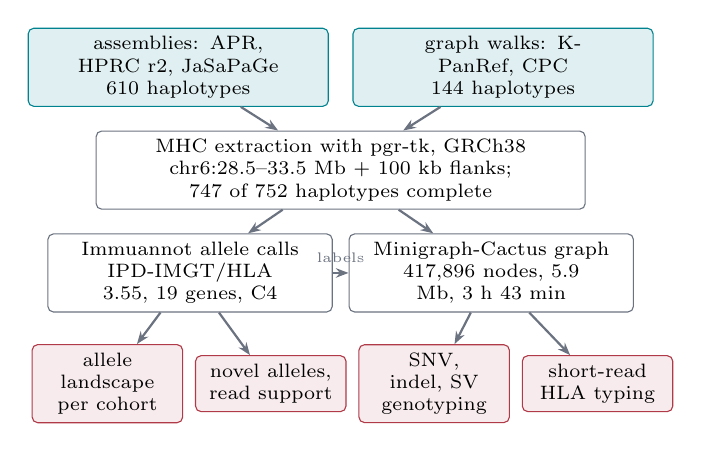
\begin{tikzpicture}[node distance=3mm and 3mm]
 \node[pdata,text width=36mm] (asm) {assemblies: APR, HPRC r2, JaSaPaGe\\ 610 haplotypes};
 \node[pdata,text width=36mm,right=of asm] (gr) {graph walks: K-PanRef, CPC\\ 144 haplotypes};
 \node[pstep,text width=60mm,below=of $(asm.south)!0.5!(gr.south)$] (ext) {MHC extraction with pgr-tk, GRCh38 chr6:28.5--33.5 Mb + 100 kb flanks; 747 of 752 haplotypes complete};
 \node[pstep,text width=34mm,below=3mm of ext.south,anchor=north east,xshift=-1mm] (imm) {Immuannot allele calls\\ IPD-IMGT/HLA 3.55, 19 genes, C4};
 \node[pstep,text width=34mm,below=3mm of ext.south,anchor=north west,xshift=1mm] (mc) {Minigraph-Cactus graph\\ 417,896 nodes, 5.9 Mb, 3 h 43 min};
 \node[pout,text width=17mm,below=4mm of imm.south west,anchor=north west,xshift=-2mm] (o1) {allele landscape per cohort};
 \node[pout,text width=17mm,right=1.5mm of o1] (o2) {novel alleles, read support};
 \node[pout,text width=17mm,right=1.5mm of o2] (o3) {SNV, indel, SV genotyping};
 \node[pout,text width=17mm,right=1.5mm of o3] (o4) {short-read HLA typing};
 \draw[arr] (asm) -- (ext); \draw[arr] (gr) -- (ext);
 \draw[arr] (ext) -- (imm); \draw[arr] (ext) -- (mc);
 \draw[arr] (imm) -- (o1); \draw[arr] (imm) -- (o2); \draw[arr] (mc) -- (o3); \draw[arr] (mc) -- (o4);
 \draw[arr,dashed] (imm.east) -- node[above,font=\tiny,grey]{labels} (mc.west);
\end{tikzpicture}
\end{column}
\begin{column}{0.42\textwidth}
\centering

\includegraphics[width=\textwidth]{fig_cohorts.png}
\end{column}
\end{columns}
\vspace{1mm}
\begin{itemize}\footnotesize
 \item Aim 1: one MHC graph that adds Arab, Saudi, Japanese, Korean and Chinese haplotypes to HPRC release 2, each labelled with full-resolution HLA alleles
 \item Aim 2: do the added haplotypes improve genotypes from 30x Illumina reads? Control: an HPRC-only panel run through the same method
 \item Aim 3: an HLA typer that names alleles and returns the full gene sequence, benchmarked against T1K and SpecHLA on 1000 Genomes donors whose own assemblies are the truth
\end{itemize}
\vfill
\src{CWL workflow on the NIG supercomputer, \texttt{github.com/leechuck/pangenome-bh26}; graph, labels and MHC reads of 2,504 1000 Genomes samples in \texttt{/home/asianhla/data/upload/HLA/}}
\end{frame}

% ------------------------------------------------------------------ slide 2
\begin{frame}{The added haplotypes improve every variant class in held-out donors, most for SVs}
\begin{columns}[T]
\begin{column}{0.46\textwidth}

\includegraphics[width=\textwidth]{fig_graph_density.png}
\end{column}
\begin{column}{0.54\textwidth}
\vspace{1mm}
\begin{itemize}\scriptsize
 \item Left: along the GRCh38 path the graph is near-linear except at HLA-A, C and B, C4, the DR-DQ block and DP; only in the DRB3/4/5 block do fewer than 60\% of haplotypes share the reference nodes. vg giraffe maps 99.5\% of one sample's MHC read pairs in 26 s
 \item Below: PanGenie 4.2.1, identical MHC reads of 40 held-out 1000 Genomes donors, truth = the donor's own assembly in the graph, test families excluded from both panels, same sites. Full vs HPRC-only: +0.1 (SNV) to +3.9 points (SV-bearing genotypes, East Asian; 95\% CI +2.4 to +5.3); on SNVs shared with the published NYGC GATK callset, +0.13 and +0.19 points over linear
\end{itemize}
\end{column}
\end{columns}
\vspace{3mm}
\centering

\includegraphics[width=0.74\textwidth]{fig_variant_classes.png}
\vfill
\src{Concordance with graph-derived assembly genotypes, not an independent truth set; panel size and ancestry are confounded (754 vs 466 haplotypes). \texttt{hla-asian50/refined/REPORT.md}}
\end{frame}

% ------------------------------------------------------------------ slide 3
\begin{frame}{Short-read HLA typing: panel wins on DRB3/4/5 and sequences, T1K on two-field names}
\centering
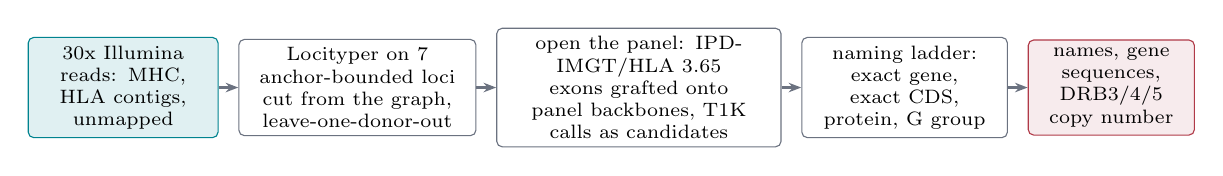
\begin{tikzpicture}[node distance=2.5mm and 2.5mm]
 \node[pdata,text width=22mm] (r) {30x Illumina reads: MHC, HLA contigs, unmapped};
 \node[pstep,text width=28mm,right=of r] (b) {Locityper on 7 anchor-bounded loci cut from the graph, leave-one-donor-out};
 \node[pstep,text width=34mm,right=of b] (c) {open the panel: IPD-IMGT/HLA 3.65 exons grafted onto panel backbones, T1K calls as candidates};
 \node[pstep,text width=24mm,right=of c] (n) {naming ladder: exact gene, exact CDS, protein, G group};
 \node[pout,text width=19mm,right=of n] (o) {names, gene sequences, DRB3/4/5 copy number};
 \draw[arr] (r)--(b); \draw[arr] (b)--(c); \draw[arr] (c)--(n); \draw[arr] (n)--(o);
\end{tikzpicture}\\[0.5mm]

\includegraphics[width=0.8\textwidth]{fig_hla_dev.png}
\begin{itemize}\scriptsize
 \item Left, 40 development donors: classical 8 genes two-field, full panel 92.5\%, Asian size-matched 92.8\%, HPRC-only 88.4\%, T1K 98.4\%; DRB3/4/5 with copy number, panel 111/113, T1K 48/110. Right: the panel in SpecHLA's read binning raises exact gene reconstructions from 41 to 51 of 128 haplotypes (HLA-B 3 to 8); names unchanged
 \item Remaining errors: DRB1 picks and alleles absent from the panel; grafted IPD exons recover 4 so far. The locked test (228 leave-one-out donors, 946 Gourraud-typed donors) has not run yet
\end{itemize}
\vfill
\src{Truth = the donor's own assembly haplotypes, IPD-IMGT/HLA 3.65.0 labels; no-calls count as errors; T1K on the same reads and database release. Code: \texttt{hla-typer/}, \texttt{hla-spechla-pg/}}
\end{frame}

\end{document}
